% Trusted Nutra Products
% ProstaPrime 30-Day Prostate Power Plan

\documentclass[11pt,oneside]{book}
\usepackage[margin=1in]{geometry}
\usepackage{titlesec}
\usepackage{graphicx}
\usepackage{array}
\usepackage{enumitem}
\usepackage{hyperref}
\usepackage{xcolor}
\usepackage{setspace}

\definecolor{brandblue}{HTML}{1565C0}

\titleformat{\chapter}{\Huge\bfseries\color{brandblue}}{}{0pt}{}
\titleformat{\section}{\Large\bfseries}{}{0pt}{}

\setlength{\parindent}{0pt}
\onehalfspacing

\begin{document}

%------------------ COVER ------------------
\pagestyle{empty}
\pagenumbering{gobble}

\begin{titlepage}
\newgeometry{margin=0pt}

\noindent
\makebox[\paperwidth][c]{%
  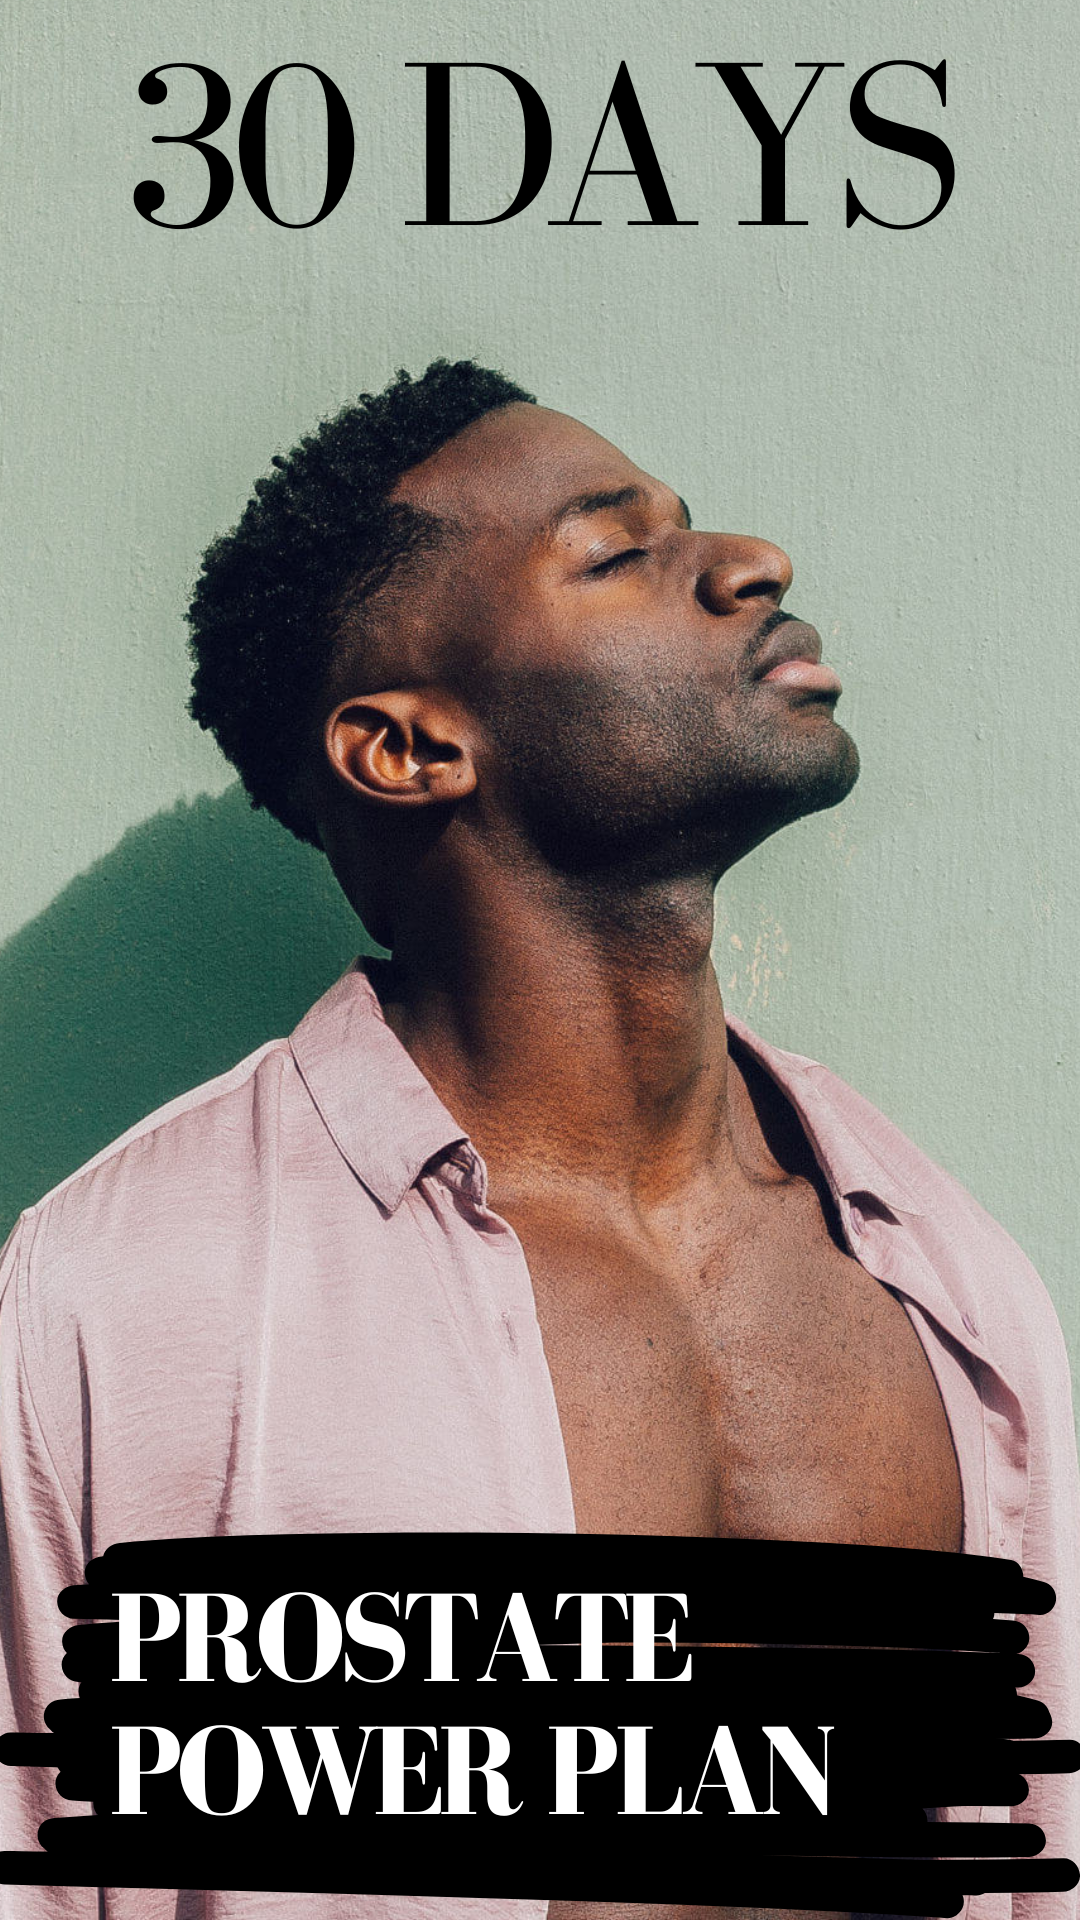
\includegraphics[
    width=\paperwidth,
    height=\paperheight
  ]{powerplan.png}%
}

\end{titlepage}

\restoregeometry
\clearpage
%---------------- END COVER ----------------


%------------------ TOC ------------------
\clearpage
\tableofcontents

\clearpage
\chapter*{Your 30-Day Prostate Power Protocol}
\addcontentsline{toc}{chapter}{Your 30-Day Prostate Power Protocol}

This isn't a diet. This isn't a quick fix. This is a complete 30-day protocol designed to rebuild your prostate health, restore bladder control, and reclaim the energy you thought was gone forever.

\textbf{The Promise:} Follow this plan for 30 days, and you WILL notice:
\begin{itemize}[leftmargin=*]
\item Fewer nighttime bathroom trips (most men drop from 3--4 to 0--1)
\item Stronger, more consistent urinary flow
\item Better bladder control throughout the day
\item Increased energy and vitality
\item Improved testosterone markers
\end{itemize}

\textbf{The Requirement:} You must commit 100\%. No half-measures. No "I'll start Monday." Today is Day 1.

\section*{ProstaPrime Daily Protocol}
\begin{itemize}[leftmargin=*]
\item \textbf{Daily dose:} 1 capsule with breakfast (follow label)
\item Full glass of water with each dose
\item Take at the same time daily for consistency
\end{itemize}

\section*{The 5 Daily Non-Negotiables}
\begin{itemize}[leftmargin=*]
\item \textbf{Strategic Hydration:} 2--3 liters daily, front-loaded before 3 PM
\item \textbf{Movement:} 30+ minutes (walking, lifting, or both)
\item \textbf{Sleep:} 7--8 hours in complete darkness
\item \textbf{Kegel Exercises:} 3 sets of 10--15 reps daily
\item \textbf{ProstaPrime:} 1 capsule daily with breakfast, no skipping
\end{itemize}

\section*{Nutrition Focus}
Every meal is strategically designed around:
\begin{itemize}[leftmargin=*]
\item \textbf{Zinc \& Selenium:} The prostate minerals (pumpkin seeds, Brazil nuts)
\item \textbf{Lycopene:} Cooked tomatoes for prostate protection
\item \textbf{Omega-3s:} Wild fish to crush inflammation
\item \textbf{Healthy Fats:} Testosterone building blocks
\item \textbf{Cruciferous Vegetables:} Estrogen metabolism support
\end{itemize}

\section*{What to Expect Week by Week}

\textbf{Week 1:} Body adjusts. You may not notice dramatic changes yet. Trust the process.

\textbf{Week 2:} First improvements. Less urgency, slightly better flow.

\textbf{Week 3:} Noticeable changes. Fewer nighttime trips, stronger stream.

\textbf{Week 4:} New baseline established. This becomes your new normal.

\textbf{Ready? Let's go.}

\clearpage
\chapter*{Day 1 – Foundation Day}
\addcontentsline{toc}{chapter}{Day 1 – Foundation Day}

\textbf{Mindset:} This is the day you take back control. No excuses, no delays.

\section*{Morning Protocol}
\begin{itemize}[leftmargin=*]
\item Wake up, drink 16 oz water immediately
\item 10--15 minutes sunlight exposure (vitamin D activation)
\item \textbf{Breakfast:} 3 eggs scrambled with spinach, tomatoes, and olive oil
\item \textbf{ProstaPrime:} 1 capsule with full glass of water
\item 1 cup green tea
\end{itemize}

\section*{Midday}
\begin{itemize}[leftmargin=*]
\item \textbf{Lunch:} Grilled wild salmon (omega-3s) with steamed broccoli (DIM)
\item \textbf{Snack:} 1/4 cup pumpkin seeds (zinc) + 3--4 Brazil nuts (selenium)
\item Hydration: Sip water throughout morning/early afternoon
\end{itemize}

\section*{Evening}
\begin{itemize}[leftmargin=*]
\item \textbf{Dinner:} Grilled chicken breast with roasted Brussels sprouts
\item Stop drinking fluids 2--3 hours before bed
\end{itemize}

\section*{Movement \& Recovery}
\begin{itemize}[leftmargin=*]
\item 30-minute brisk walk (aim for 10,000 steps)
\item Kegel exercises: 3 sets of 15 reps (morning, afternoon, evening)
\item Cold shower finish: 30--60 seconds
\item 10 minutes light stretching before bed
\end{itemize}

\section*{Track This}
\begin{itemize}[leftmargin=*]
\item How many times did you urinate during the night? \_\_\_\_
\item Urinary flow: Weak / Moderate / Strong (circle one)
\item Energy level (1--10): \_\_\_\_
\end{itemize}

\clearpage
\chapter*{Day 2 – Build the Foundation}
\addcontentsline{toc}{chapter}{Day 2 – Build the Foundation}

\section*{What to Eat}
\begin{itemize}[leftmargin=*]
\item Breakfast: Greek yogurt with blueberries and walnuts
\item Lunch: Quinoa bowl with grilled chicken and avocado
\item Snack: Apple slices with almond butter
\item Dinner: Baked cod with asparagus
\end{itemize}

\section*{What to Drink}
\begin{itemize}[leftmargin=*]
\item 2.5--3 liters water (limit after 6 PM)
\item Herbal tea (optional)
\end{itemize}

\section*{What to Do}
\begin{itemize}[leftmargin=*]
\item 25-minute walk
\item Kegel exercises (3 sets)
\item 5 minutes deep breathing
\end{itemize}

\section*{ProstaPrime}
1 capsule with breakfast.

\clearpage
\chapter*{Day 3 – Steady Progress}
\addcontentsline{toc}{chapter}{Day 3 – Steady Progress}

\section*{What to Eat}
\begin{itemize}[leftmargin=*]
\item Breakfast: Omelet with tomatoes, onions, and bell peppers
\item Lunch: Turkey and avocado wrap (whole wheat)
\item Snack: Brazil nuts (3--4 nuts for selenium)
\item Dinner: Grilled chicken with roasted cauliflower
\end{itemize}

\section*{What to Drink}
Water throughout the day (front-load morning).

\section*{What to Do}
30 minutes steady walking, Kegel exercises.

\section*{ProstaPrime}
Continue daily dosage.

\clearpage
\chapter*{Day 4 – Anti-Inflammatory Focus}
\addcontentsline{toc}{chapter}{Day 4 – Anti-Inflammatory Focus}

\section*{What to Eat}
\begin{itemize}[leftmargin=*]
\item Breakfast: Smoothie (spinach, berries, protein powder)
\item Lunch: Lentil soup with side salad
\item Snack: Carrot sticks with hummus
\item Dinner: Baked salmon with green beans
\end{itemize}

\section*{What to Drink}
2.5--3 liters water, 1 cup green tea.

\section*{What to Do}
Gentle yoga or stretching (20 minutes), Kegels.

\section*{ProstaPrime}
Take as directed.

\clearpage
\chapter*{Day 5 – Power Foods}
\addcontentsline{toc}{chapter}{Day 5 – Power Foods}

\section*{What to Eat}
\begin{itemize}[leftmargin=*]
\item Breakfast: Oatmeal with chia seeds and berries
\item Lunch: Grilled mackerel with mixed greens
\item Snack: Pumpkin seeds
\item Dinner: Turkey meatballs with marinara (extra tomatoes)
\end{itemize}

\section*{What to Drink}
2.5--3 liters water.

\section*{What to Do}
30-minute brisk walk, Kegel exercises.

\section*{ProstaPrime}
Continue daily dosage.

\clearpage
\chapter*{Day 6 – Active Recovery}
\addcontentsline{toc}{chapter}{Day 6 – Active Recovery}

\section*{What to Eat}
\begin{itemize}[leftmargin=*]
\item Breakfast: 2 poached eggs with avocado
\item Lunch: Chicken salad with olive oil dressing
\item Snack: Mixed nuts (almonds, walnuts)
\item Dinner: Grilled shrimp with zucchini
\end{itemize}

\section*{What to Drink}
Water + optional herbal tea.

\section*{What to Do}
Stretching + 20-minute walk, Kegels.

\section*{ProstaPrime}
Take as directed.

\clearpage
%======================
% PART 2: DAYS 7–12
%======================

\chapter*{Day 7 – Week 1 Complete: Assessment Day}
\addcontentsline{toc}{chapter}{Day 7 – Week 1 Complete}

\textbf{Congratulations.} You just completed the hardest week. Your body is adapting. Changes are happening at the cellular level even if you don't feel them yet.

\section*{Today's Meals}
\begin{itemize}[leftmargin=*]
\item \textbf{Breakfast:} Greek yogurt with flaxseeds, berries, walnuts
\item \textbf{Lunch:} Baked chicken with roasted vegetables (include tomatoes)
\item \textbf{Snack:} Apple slices with almond butter
\item \textbf{Dinner:} Tomato-based vegetable soup with lean protein
\end{itemize}

\section*{Week 1 Progress Check}

\textbf{Answer These Honestly:}

\textbf{1. Nighttime Urination}
\begin{itemize}[leftmargin=*]
\item Day 1 trips: \_\_\_\_ | Day 7 trips: \_\_\_\_
\item Improvement? Yes / No / Slight
\end{itemize}

\textbf{2. Urinary Flow Strength}
\begin{itemize}[leftmargin=*]
\item Day 1: Weak / Moderate / Strong
\item Day 7: Weak / Moderate / Strong
\item Improvement? Yes / No / Slight
\end{itemize}

\textbf{3. Urgency \& Control}
\begin{itemize}[leftmargin=*]
\item Fewer sudden urges? Yes / No / About the same
\item Better control when urge hits? Yes / No / About the same
\end{itemize}

\textbf{4. Energy Levels}
\begin{itemize}[leftmargin=*]
\item Day 1 (1--10): \_\_\_\_ | Day 7 (1--10): \_\_\_\_
\end{itemize}

\textbf{5. Compliance Check}
\begin{itemize}[leftmargin=*]
\item ProstaPrime taken daily? \_\_\_/7 days
\item Kegels completed daily? \_\_\_/7 days
\item Hit movement goals? \_\_\_/7 days
\item Front-loaded hydration? \_\_\_/7 days
\end{itemize}

\section*{Week 1 Lessons}

\textbf{What worked well this week?}

\vspace{2cm}

\textbf{What needs adjustment?}

\vspace{2cm}

\textbf{Commitment for Week 2:}

\vspace{2cm}

\section*{Movement Today}
\begin{itemize}[leftmargin=*]
\item Light 20--30 minute recovery walk
\item Kegel exercises (3 sets)
\item Stretching or yoga (20 minutes)
\item Reflect and plan Week 2
\end{itemize}

\textbf{Reminder:} Week 2 is where real changes accelerate. Stay the course.

\clearpage


\chapter*{Day 8 – Omega-3 Boost}
\addcontentsline{toc}{chapter}{Day 8 – Omega-3 Boost}

\section*{What to Eat}
\begin{itemize}[leftmargin=*]
\item Breakfast: Scrambled eggs with smoked salmon
\item Lunch: Tuna salad with olive oil and greens
\item Snack: Walnuts
\item Dinner: Baked trout with steamed broccoli
\end{itemize}

\section*{What to Drink}
Water throughout the day + 1 cup green tea.

\section*{What to Do}
30-minute brisk walk, light stretching, Kegels.

\section*{ProstaPrime}
Continue daily dosage.

\clearpage


\chapter*{Day 9 – Lycopene Power}
\addcontentsline{toc}{chapter}{Day 9 – Lycopene Power}

\section*{What to Eat}
\begin{itemize}[leftmargin=*]
\item Breakfast: Omelet with tomatoes and onions
\item Lunch: Chicken with tomato-based sauce
\item Snack: Cherry tomatoes with mozzarella
\item Dinner: Grilled fish with roasted red peppers
\end{itemize}

\section*{What to Drink}
Minimum 2.5 liters water.

\section*{What to Do}
35-minute walk or light cardio, Kegels.

\section*{ProstaPrime}
Take as directed with meals.

\clearpage


\chapter*{Day 10 – Consistency Day}
\addcontentsline{toc}{chapter}{Day 10 – Consistency Day}

\section*{What to Eat}
\begin{itemize}[leftmargin=*]
\item Breakfast: Smoothie (spinach, berries, protein)
\item Lunch: Quinoa with grilled vegetables
\item Snack: Pumpkin seeds
\item Dinner: Turkey breast with green beans
\end{itemize}

\section*{What to Drink}
2.5--3 liters water, avoid sugary drinks.

\section*{What to Do}
30 minutes walking + 5 minutes breathing exercises, Kegels.

\section*{ProstaPrime}
Continue as directed.

\clearpage


\chapter*{Day 11 – Cruciferous Power}
\addcontentsline{toc}{chapter}{Day 11 – Cruciferous Power}

\section*{What to Eat}
\begin{itemize}[leftmargin=*]
\item Breakfast: Eggs with sautéed kale
\item Lunch: Grilled chicken with cauliflower rice
\item Snack: Brazil nuts (3--4)
\item Dinner: Baked salmon with Brussels sprouts
\end{itemize}

\section*{What to Drink}
Water all day, herbal tea optional.

\section*{What to Do}
Gentle yoga or stretching (25 minutes), Kegels.

\section*{ProstaPrime}
Take as directed.

\clearpage


\chapter*{Day 12 – Momentum Builder}
\addcontentsline{toc}{chapter}{Day 12 – Momentum Builder}

\section*{What to Eat}
\begin{itemize}[leftmargin=*]
\item Breakfast: Greek yogurt with berries and chia
\item Lunch: Tuna wrap with avocado
\item Snack: Mixed nuts
\item Dinner: Grilled turkey with roasted vegetables
\end{itemize}

\section*{What to Drink}
3 liters water, green tea optional.

\section*{What to Do}
40-minute brisk walk, Kegels.

\section*{ProstaPrime}
Continue daily dosage.

\clearpage
%======================
% PART 3: DAYS 13–18
%======================

\chapter*{Day 13 – Halfway Point: Momentum Check}
\addcontentsline{toc}{chapter}{Day 13 – Halfway Point}

\textbf{You're officially halfway.} This is where quitters drop out. This is where champions double down.

Which one are you?

\section*{Today's Protocol}
\begin{itemize}[leftmargin=*]
\item \textbf{Breakfast:} 2--3 boiled eggs with tomato slices and avocado
\item \textbf{Lunch:} Grilled wild salmon with mixed greens and olive oil
\item \textbf{Snack:} 1/4 cup pumpkin seeds + 3--4 Brazil nuts
\item \textbf{Dinner:} Grilled chicken breast with steamed broccoli
\item \textbf{Hydration:} 2.5--3 liters, front-loaded before 3 PM
\item \textbf{ProstaPrime:} 1 capsule with breakfast
\end{itemize}

\section*{Midpoint Performance Review}

\textbf{Nighttime Freedom Progress}
\begin{itemize}[leftmargin=*]
\item Week 1 average (Days 1--7): \_\_\_\_ trips
\item Week 2 average (Days 8--13): \_\_\_\_ trips
\item Improvement: \_\_\_\_ fewer trips per night
\item Sleeping 4+ hours straight? Yes / No / Sometimes
\end{itemize}

\textbf{Daytime Function}
\begin{itemize}[leftmargin=*]
\item Urination frequency: Every \_\_\_\_ hours
\item Stream strength: Weak / Moderate / Strong
\item Urgency reduced? Yes / No / Somewhat
\item Bladder emptying: Complete / Mostly / Incomplete
\end{itemize}

\textbf{Energy \& Vitality}
\begin{itemize}[leftmargin=*]
\item Morning energy (1--10): \_\_\_\_
\item Afternoon energy (1--10): \_\_\_\_
\item Overall stamina: Improved / Same / Worse
\end{itemize}

\textbf{Honest Compliance Check}
\begin{itemize}[leftmargin=*]
\item ProstaPrime taken daily: \_\_\_\_/13 days
\item Kegel exercise days: \_\_\_\_/13
\item Movement/exercise days: \_\_\_\_/13
\item Clean eating days: \_\_\_\_/13
\item Hydration protocol followed: \_\_\_\_/13
\end{itemize}

\section*{Course Correction (If Needed)}

\textbf{If you're seeing results:} Keep doing exactly what you're doing.

\textbf{If progress is slow:}
\begin{itemize}[leftmargin=*]
\item Are you REALLY front-loading water before 3 PM?
\item Are you doing Kegels EVERY day (not just "when you remember")?
\item Is your ProstaPrime dosing consistent (same times daily)?
\item Are you eating enough zinc and selenium foods?
\item Are you eliminating bladder irritants (caffeine, alcohol)?
\end{itemize}

\section*{Movement \& Mindset}
\begin{itemize}[leftmargin=*]
\item 30--40 minute brisk walk or strength training
\item Kegel exercises: 3 sets of 15 reps
\item 10 minutes stretching
\item Reflect: What's working? What needs adjustment?
\end{itemize}

\textbf{The Second Half:} This is where the magic happens. Your body is primed. Your habits are forming. Push harder.

\clearpage


\chapter*{Day 14 – Anti-Inflammatory Day}
\addcontentsline{toc}{chapter}{Day 14 – Anti-Inflammatory Day}

\section*{What to Eat}
\begin{itemize}[leftmargin=*]
\item Breakfast: Smoothie bowl with berries and nuts
\item Lunch: Mackerel with steamed vegetables
\item Snack: Apple with almond butter
\item Dinner: Turkey meatballs with marinara
\end{itemize}

\section*{What to Drink}
Water throughout the day (minimum 2.5 liters).

\section*{What to Do}
35-minute walk or light cardio, Kegels.

\section*{ProstaPrime}
Continue daily dosage.

\clearpage


\chapter*{Day 15 – Strong & Steady}
\addcontentsline{toc}{chapter}{Day 15 – Strong & Steady}

\section*{What to Eat}
\begin{itemize}[leftmargin=*]
\item Breakfast: Omelet with spinach and mushrooms
\item Lunch: Chicken and vegetable bowl
\item Snack: Walnuts
\item Dinner: Grilled cod with asparagus
\end{itemize}

\section*{What to Drink}
2.5--3 liters water, avoid caffeine after 2 PM.

\section*{What to Do}
40-minute brisk walk, Kegels.

\section*{ProstaPrime}
Take as directed.

\clearpage


\chapter*{Day 16 – Active Recovery}
\addcontentsline{toc}{chapter}{Day 16 – Active Recovery}

\section*{What to Eat}
\begin{itemize}[leftmargin=*]
\item Breakfast: Greek yogurt with flaxseeds
\item Lunch: Grilled fish with salad
\item Snack: Brazil nuts (3--4)
\item Dinner: Steamed vegetables with lean protein
\end{itemize}

\section*{What to Drink}
Water all day, herbal tea optional.

\section*{What to Do}
Gentle yoga or stretching (30 minutes), Kegels.

\section*{ProstaPrime}
Continue as directed.

\clearpage


\chapter*{Day 17 – Nutrient Dense}
\addcontentsline{toc}{chapter}{Day 17 – Nutrient Dense}

\section*{What to Eat}
\begin{itemize}[leftmargin=*]
\item Breakfast: Scrambled eggs with tomatoes and avocado
\item Lunch: Salmon salad with olive oil
\item Snack: Pumpkin seeds
\item Dinner: Grilled chicken with roasted peppers
\end{itemize}

\section*{What to Drink}
3 liters water, green tea optional.

\section*{What to Do}
45-minute walk or light cardio, Kegels.

\section*{ProstaPrime}
Take as directed.

\clearpage


\chapter*{Day 18 – Progress Check}
\addcontentsline{toc}{chapter}{Day 18 – Progress Check}

\section*{What to Eat}
\begin{itemize}[leftmargin=*]
\item Breakfast: Smoothie (greens, berries, protein)
\item Lunch: Turkey and avocado wrap
\item Snack: Mixed nuts
\item Dinner: Baked fish with green beans
\end{itemize}

\section*{What to Drink}
2.5--3 liters water.

\section*{What to Do}
30-minute walk + 10 minutes stretching, Kegels.

\section*{ProstaPrime}
Continue daily dosage.

\clearpage
%======================
% PART 4: DAYS 19–30
%======================

\chapter*{Day 19 – Consistency Wins}
\addcontentsline{toc}{chapter}{Day 19 – Consistency Wins}

\section*{What to Eat}
Eggs with vegetables (breakfast), grilled chicken salad (lunch), pumpkin seeds (snack), salmon with broccoli (dinner).

\section*{What to Drink}
2.5--3 liters water.

\section*{What to Do}
30-minute brisk walk, Kegels.

\section*{ProstaPrime}
Take as directed.

\clearpage


\chapter*{Day 20 – Light & Clean}
\addcontentsline{toc}{chapter}{Day 20 – Light & Clean}

\section*{What to Eat}
Greek yogurt with berries, tuna salad, apple with nuts, grilled turkey with vegetables.

\section*{What to Do}
Stretching + 25-minute walk, Kegels.

\section*{ProstaPrime}
Continue daily dosage.

\clearpage


\chapter*{Day 21 – Three-Week Milestone: The Transformation Zone}
\addcontentsline{toc}{chapter}{Day 21 – Three-Week Milestone}

\textbf{This is it.} You're in the zone where habits become automatic and results become undeniable. Most men quit before they reach this point. You didn't. That says everything.

\section*{Today's Nutrition}
\begin{itemize}[leftmargin=*]
\item \textbf{Breakfast:} Omelet (3 eggs) with tomatoes, onions, spinach
\item \textbf{Lunch:} Chicken and quinoa bowl with avocado and greens
\item \textbf{Snack:} Mixed nuts (pumpkin seeds, almonds, walnuts)
\item \textbf{Dinner:} Hearty vegetable soup with lean protein
\end{itemize}

\section*{3-Week Transformation Assessment}

\textbf{Nighttime Freedom}
\begin{itemize}[leftmargin=*]
\item Day 1 average trips: \_\_\_\_ | Day 21 average: \_\_\_\_
\item Reduction: \_\_\_\_ trips per night
\item Sleeping through the night? Yes / No / Sometimes
\end{itemize}

\textbf{Urinary Function}
\begin{itemize}[leftmargin=*]
\item Stream strength improved? Yes / No / Significantly
\item Hesitancy reduced? Yes / No
\item Post-void dribbling better? Yes / No
\item Overall bladder control (1--10): \_\_\_\_
\end{itemize}

\textbf{Energy \& Vitality}
\begin{itemize}[leftmargin=*]
\item Morning energy (1--10): \_\_\_\_
\item Overall stamina: Better / Same / Worse
\item Mood and confidence: Improved / Same / Worse
\end{itemize}

\textbf{Physical Changes}
\begin{itemize}[leftmargin=*]
\item Weight change: +/- \_\_\_\_ lbs
\item Muscle tone: Better / Same / Worse
\item Inflammation/bloating: Reduced / Same / Increased
\end{itemize}

\textbf{Compliance Score (Be Honest)}
\begin{itemize}[leftmargin=*]
\item ProstaPrime daily: \_\_\_/21 days
\item Kegel exercises: \_\_\_/21 days
\item Movement goals: \_\_\_/21 days
\item Nutrition compliance: \_\_\_/21 days
\item Hydration protocol: \_\_\_/21 days
\end{itemize}

\section*{What's Changed Mentally?}

\textbf{List 3 ways you feel different than Day 1:}

1. \underline{\hspace{10cm}}

2. \underline{\hspace{10cm}}

3. \underline{\hspace{10cm}}

\section*{Movement \& Recovery}
\begin{itemize}[leftmargin=*]
\item Gentle yoga or active recovery (30 minutes)
\item Kegel exercises (3 sets of 15 reps)
\item Nature walk or outdoor activity
\item Deep breathing and reflection
\end{itemize}

\textbf{Final 9 Days:} This is where you cement these changes for life. Finish strong.

\clearpage


\chapter*{Day 22 – Antioxidant Boost}
\addcontentsline{toc}{chapter}{Day 22 – Antioxidant Boost}

\section*{What to Eat}
Berry smoothie, grilled fish with tomato sauce, walnuts, chicken with roasted vegetables.

\section*{What to Do}
40-minute brisk walk, Kegels.

\section*{ProstaPrime}
Take as directed.

\clearpage


\chapter*{Day 23 – Strong Habits}
\addcontentsline{toc}{chapter}{Day 23 – Strong Habits}

\section*{What to Eat}
Eggs and avocado, salmon with greens, Brazil nuts, turkey with Brussels sprouts.

\section*{What to Do}
30--40 minutes walking, Kegels.

\section*{ProstaPrime}
Continue daily use.

\clearpage


\chapter*{Day 24 – Light & Balanced}
\addcontentsline{toc}{chapter}{Day 24 – Light & Balanced}

\section*{What to Eat}
Oatmeal with seeds, grilled chicken with vegetables, fruit, steamed greens with fish.

\section*{What to Do}
Stretching + breathing exercises, Kegels.

\section*{ProstaPrime}
As directed.

\clearpage


\chapter*{Day 25 – Stay the Course}
\addcontentsline{toc}{chapter}{Day 25 – Stay the Course}

\section*{What to Eat}
Scrambled eggs, tuna salad, pumpkin seeds, chicken with cauliflower.

\section*{What to Do}
45-minute walk, Kegels.

\section*{ProstaPrime}
Take as directed.

\clearpage


\chapter*{Day 26 – Mindful Nutrition}
\addcontentsline{toc}{chapter}{Day 26 – Mindful Nutrition}

\section*{What to Eat}
Greek yogurt with berries, baked salmon with salad, mixed nuts, turkey with greens.

\section*{What to Do}
Eat slowly, 30-minute walk, Kegels.

\section*{ProstaPrime}
Continue daily dosage.

\clearpage


\chapter*{Day 27 – Energy \& Focus}
\addcontentsline{toc}{chapter}{Day 27 – Energy \& Focus}

\section*{What to Eat}
Smoothie, grilled fish with vegetables, Brazil nuts, chicken with roasted peppers.

\section*{What to Do}
40 minutes brisk walking, Kegels.

\section*{ProstaPrime}
As directed.

\clearpage


\chapter*{Day 28 – The Final Sprint}
\addcontentsline{toc}{chapter}{Day 28 – The Final Sprint}

\textbf{Two days left.} This is where champions prove themselves. Go all-in today.

\section*{Peak Performance Nutrition}
\begin{itemize}[leftmargin=*]
\item \textbf{Breakfast:} 3 eggs scrambled with spinach, tomatoes, avocado
\item \textbf{Lunch:} Wild salmon salad with mixed greens, olive oil, pumpkin seeds
\item \textbf{Snack:} Brazil nuts (3--4) + walnuts
\item \textbf{Dinner:} Grilled turkey breast with steamed green beans and Brussels sprouts
\item \textbf{ProstaPrime:} 1 capsule daily with breakfast, no skipping
\end{itemize}

\section*{Maximum Effort Day}
\begin{itemize}[leftmargin=*]
\item 45--60 minute walk or strength training session
\item Kegel exercises: 4 sets of 15--20 reps (push harder)
\item Cold shower finish: 2--3 minutes (testosterone boost)
\item 15 minutes stretching or yoga
\end{itemize}

\section*{Pre-Finish Line Check}

\textbf{Rate yourself honestly (1--10):}
\begin{itemize}[leftmargin=*]
\item Nighttime urination improvement: \_\_\_\_
\item Daytime bladder control: \_\_\_\_
\item Urinary flow strength: \_\_\_\_
\item Overall energy: \_\_\_\_
\item Confidence level: \_\_\_\_
\item Commitment to continue: \_\_\_\_
\end{itemize}

\textbf{Tomorrow:} Day 29 is your recovery day. Prepare mentally for Day 30's final assessment.

\textbf{Reminder:} These final days cement the changes. Don't coast to the finish line—sprint through it.

\clearpage


\chapter*{Day 29 – Light Day}
\addcontentsline{toc}{chapter}{Day 29 – Light Day}

\section*{What to Eat}
Light meals: vegetable soups, salads, lean protein, extra hydration.

\section*{What to Drink}
Extra hydration (3 liters, but reduce evening intake).

\section*{What to Do}
Gentle walking, deep breathing, Kegels.

\section*{ProstaPrime}
Continue daily dosage.

\clearpage


\chapter*{Day 30 – Mission Complete: Your New Baseline}
\addcontentsline{toc}{chapter}{Day 30 – Mission Complete}

\textbf{You did it.}

30 days of commitment. 30 days of discipline. 30 days of taking control when most men just accept decline.

This isn't the end. This is your new beginning.

\section*{Final Assessment: Where You Stand}

\textbf{The Numbers}

\textit{Nighttime Urination}
\begin{itemize}[leftmargin=*]
\item Day 1 baseline: \_\_\_\_ trips per night
\item Day 30 result: \_\_\_\_ trips per night
\item Total reduction: \_\_\_\_ trips (\_\_\_\% improvement)
\end{itemize}

\textit{Urinary Function}
\begin{itemize}[leftmargin=*]
\item Stream strength: Weak / Moderate / Strong / Very Strong
\item Start time (hesitancy): Immediate / Slight delay / Long delay
\item Bladder emptying: Complete / Mostly / Incomplete
\item Overall control (1--10): \_\_\_\_
\end{itemize}

\textit{Physical Transformation}
\begin{itemize}[leftmargin=*]
\item Weight change: +/- \_\_\_\_ lbs
\item Energy level (1--10): \_\_\_\_
\item Sleep quality (1--10): \_\_\_\_
\item Confidence (1--10): \_\_\_\_
\end{itemize}

\section*{What You've Proven}

You've proven that prostate health ISN'T just "part of getting older."

You've proven that natural solutions WORK when applied consistently.

You've proven that YOU control your health outcomes.

\section*{Biggest Wins (List 5)}

1. \underline{\hspace{10cm}}

2. \underline{\hspace{10cm}}

3. \underline{\hspace{10cm}}

4. \underline{\hspace{10cm}}

5. \underline{\hspace{10cm}}

\section*{Your Next 30 Days}

This protocol doesn't end today. These habits are now your lifestyle.

\textbf{Continue:}
\begin{itemize}[leftmargin=*]
\item ProstaPrime daily (ongoing support)
\item Prostate-friendly nutrition (zinc, selenium, lycopene, omega-3s)
\item Strategic hydration (front-load, stop 2--3 hours before bed)
\item Daily movement and strength training
\item Kegel exercises (maintain pelvic floor strength)
\item Quality sleep in complete darkness
\end{itemize}

\textbf{Add:}
\begin{itemize}[leftmargin=*]
\item Quarterly prostate check-ups (stay proactive)
\item Advanced strength training (build more muscle = more testosterone)
\item Stress management practices (meditation, nature time)
\item Community support (share your wins, help other men)
\end{itemize}

\section*{Warning: The 70/30 Rule}

You need 70\% compliance to MAINTAIN results.

You need 90\%+ compliance to IMPROVE further.

Slipping back to old habits = slipping back to old problems.

\textbf{Your choice.}

\section*{Today's Celebration Meal}

Eat clean, but enjoy the food that fueled your transformation:
\begin{itemize}[leftmargin=*]
\item Grass-fed steak or wild salmon
\item Roasted vegetables with olive oil
\item Sweet potato or quinoa
\item Dark chocolate (85\%+ cacao) for dessert
\end{itemize}

\section*{Final Words}

You just did what 95\% of men never do: you took action, stayed consistent, and saw it through.

Your prostate health has improved.

Your energy has returned.

Your confidence is back.

\textbf{This is your new normal. Protect it.}

Welcome to the 5\%.

\clearpage


\chapter*{The Brotherhood of Men Who Don't Settle}
\addcontentsline{toc}{chapter}{The Brotherhood of Men Who Don't Settle}

You just joined an elite group: men who refuse to accept decline as inevitable.

Men who take action instead of complaining.

Men who choose discipline over comfort.

Men who understand that health is the foundation of everything else in life.

\section*{The Path Forward}

This 30-day protocol gave you the blueprint. Now you own it.

\textbf{Keep doing what works:}
\begin{itemize}[leftmargin=*]
\item ProstaPrime daily (your prostate's insurance policy)
\item Zinc and selenium every day (pumpkin seeds, Brazil nuts)
\item Lycopene from cooked tomatoes (prostate protection)
\item Omega-3s from wild fish (crush inflammation)
\item Strategic hydration (front-load water, dry before bed)
\item Strength training 3--4x weekly (testosterone optimization)
\item Kegel exercises daily (bladder control maintenance)
\item 7--8 hours of quality sleep (recovery and hormones)
\end{itemize}

\textbf{Avoid what destroys:}
\begin{itemize}[leftmargin=*]
\item Plastics and BPA (hormone disruptors)
\item Processed foods and sugar (inflammation triggers)
\item Excessive alcohol (testosterone killer)
\item Chronic stress (cortisol elevation)
\item Sedentary lifestyle (circulation destroyer)
\end{itemize}

\section*{Share Your Wins}

Other men are struggling right now with the same issues you just conquered.

Your success can inspire them to take action.

Share what worked. Help another man reclaim his health.

\section*{Stay Connected}

Visit \textbf{TrustedNutraProducts.com} for:
\begin{itemize}[leftmargin=*]
\item Additional resources and guides
\item Ongoing support and community
\item Advanced protocols and strategies
\item ProstaPrime restocking
\end{itemize}

\section*{Remember This}

Every man over 40 faces a choice:

Accept decline, or fight back with everything you've got.

You chose to fight.

You committed 30 days.

You saw results.

\textbf{Don't stop now.}

\vspace{1cm}

\section*{Disclaimer}
This 30-day plan is intended for educational purposes only and does not replace professional medical advice, diagnosis, or treatment. Always consult a qualified healthcare provider before making dietary changes, starting an exercise program, or beginning any supplement regimen. ProstaPrime is a dietary supplement and is not intended to diagnose, treat, cure, or prevent any disease. Individual results may vary based on health status, lifestyle factors, and adherence to the protocol.

\vspace{1.5cm}

\begin{center}
\large\textbf{Here's to reclaimed vitality, restored confidence,}

\large\textbf{and refusing to settle for less.}

\vspace{0.5cm}

\textit{— TrustedNutraProducts Team}
\end{center}

\end{document}
